\chapter{backchan.nl}
\label{ch:backchannl}

In this chapter, we describe \emph{backchan.nl}, a web-based system that focuses on providing greater audience participation during question and answer sessions. The system allows audience members to propose questions and comments, and to vote on the questions of others. Top rated submissions are projected into the presentation space where audience members, moderators, and panelists can see them. We discuss the results of deploying this system at many different kinds of conferences and relate those results to the particular design of our system, demonstrating how systems for audience participation can be more than just shared chat rooms. From our experience with this work, we discuss the broader implications of configurable mediated social spaces and how subtle design decisions can influence user experience. \sidenote{The project name \emph{backchan.nl} is rather confusing in light of my refutation of the front channel/back channel distinction. This work pre-dated that framing, and when this project was named I still viewed my goal as creating a useful backchannel experience. Despite this, this project represented progress towards the development of the notion of stages, and so I have updated its language and analysis to reflect this shift.}

\section{Introduction}
The utility of computer mediated communication techniques to provide a sort of ``backchannel'' to some other conversation has been demonstrated in a few different venues, most commonly in conferences \citep{mccarthy_digital_2004, Rekimoto:1998jy} and classrooms \citep{Cogdill:2001fp, Yardi:2006uk}. Most backchannels have been text based chat or instant messaging systems that support a dialog between people who are co-present in a real world space having some sort of shared experience. The challenge with backchannels is their covert nature. The backchannels in conferences and classroom contexts are usually not accessible to the presenter, and instead focus on creating conversation within the audience. We think of this configuration not as a front channel and a back channel, but as a main stage (the audio and visual components of the presentation) and a side stage we designed to support intra audience interaction and audience-presenter interaction.

In this project, we propose a design that, rather than relying on chat, lets participants pose questions or comments to presenters, moderators, or participants in a public discussion, which can then be voted on by other audience members. The top posts are projected on a screen to the side of the presenter's table, visible by the audience. This focus on posting specific questions and not on supporting dialog creates a focused environment that is less about connecting audience members with each other, and much more about making sure popular questions get asked of the presenters in the often limited question-and-answer period. We see this as a valuable alternative to traditional question asking procedures, which favor those audience members who are most vocal or who happen to be seated near a microphone (or those familiar with the moderator, panelists or organization hosting the event). Furthermore, should the format of the event allow, this system enables moderators and panelists to address key concerns as they occur without the potential interruption of taking questions throughout. Finally, this project demonstrates audience interactions during live events need not be limited to chat nor take place in separate spaces from the main discussion; we can imagine a wide variety of tools that support interaction between co-present people focused on different goals.

\section{Related Work}

The phrase ``backchannel'' has historically referred not to mediated communication at all, but the verbal and non-verbal cues that non-speakers give a speaker during a conversation. Non-lexical utterances such as ``uh-huh'' and ``sure'', or body language cues such as shaking your head or averting your gaze all provide meaningful and important feedback to a speaker without necessarily trying to take a turn speaking. Audible and non-audible signals have both been shown to be important for maintaining communication efficiency by \citet{Krauss:1977bu}. Use of ``backchannel'' to describe these actions suggests developing non-primary communication channels between speakers and listeners can be a powerful way to create more effective conversation spaces. This metaphor has been extended in the literature to include any system in which there is an additional mediated channel separate from the primary channel of communication (which may itself be mediated). Such systems often serve to connect groups of listeners to a single speaker, though other configurations are certainly possible. Although this term represents the chat-oriented, audience-only systems discussed in this section, we view our work as being in a separate category of systems that aim instead to create a side stage that complements the main stage experience. 

There are two main approaches to understanding backchannel use in past projects. The first focuses on existing chat or instant messaging tools, and examine the type of communication that takes place on these channels and the relationship between this communication, the users of the backchannel, and the presentation they are participating in.

Based on IRC logs recorded during a conference, \citet{mccarthy_digital_2004} explores the kinds of conversations that took place and the relative involvement of different users, to propose a general taxonomy of the kinds of conversations held. This approach is similar to \citet{Yardi:2006uk}, who describes the use of an IRC backchannel in a higher education environment. Both projects build models that describe the kinds of messages that happen on backchannels. Yardi in particular focuses on the ways that over time, participants in the backchannel develop both fluency with the tool and community standards for its use.

\citet{Ratto:2003vs} discuss their experience deploying the \emph{ActiveClassroom} tool, which (like ours) lets students post and vote on questions. Their interaction is PDA based, and is not projected in the space---instead giving all moderation control to the teacher. Their analysis focuses on one semester long class, and presents little quantitative usage data to drive their analysis.

\citet{Golub:2005ws} discusses the tension between the utility of backchannels (and internet access in general) during a presentation and provides observations of what audience-members use laptops for during presentations.

Backchannels have also been proposed in the audio domain, in which members of an audio conference can create sub-conferences separate from the main shared audio channel. \citep{Yankelovich:2005bx}

Our work contrasts with these examples because we focus on posts instead of a live chat space and making the contents of that space visible to presenters and the audience, our work shows how the contents of a side stage-style system can be more effectively integrated into physical presentation spaces. 

The second approach examines backchannels as an augmentation of physical spaces to create new social environments. These projects seek to connect multiple physical spaces \citep{Karahalios:2004eg} or alter the interpersonal dynamics in a space by visualizing aspects of the conversation \citep{DiMicco:2007ie,Donath:1999kw,Bergstrom:2007je}, which start to point in the direction of a side stage approach. These systems are focused on one-to-one or small group interactions instead of connecting large audiences with a small number of presenters. At this scale of interaction, the value of a side stage diminishes because participation on the main stage is easier and more equitable. 

The work of \citet{Rekimoto:1998jy} combines elements of these two approaches by making the contents of a backchannel chat channel visible on a screen to the side of the presentation slides, though the rate of chat messages makes it hard for the audience to engage with its contents. 

At the 1988 Junior Summit, participants were given two-way pagers that could send messages to a scrolling LED text screen in an auditorium. Much like in our system, while the students found the system empowering and engaging, the organizers struggled with identity, moderation, and accountability issues. Unfortunately, there is little data available about this particular deployment. \citep{Chesnais:uh}

A very similar tool has been produced by the Berkman Center at Harvard University for classroom use. Although we were not aware of it during development, our designs are broadly similar. Source code for this tool is available online. \citep{Anonymous:DYsIxdHV} Question Tool's primary difference is that it is not designed to play a major visual role in the classroom. Students can use it as a sort of guided discussion space and teaching assistants are often present to answer some questions, but it doesn't have a distinct public projection view. The view that students use to interact with it can be projected (and sometimes is), but the system is not designed specifically with that use in mind. As a result, the tool is generally effective at creating a side stage experience but has trouble merging that experience with the main stage in some situations. 


\section{Design}

Backchan.nl is a web-based system for posting text items (nominally questions, but any text could be posted) and voting on other people's submissions. Audience members participate by visiting the \emph{backchan.nl} website on their laptops. Posts can be voted either up or down, and are ranked using a formula that rewards positive votes, a high volume of votes, and recent votes. The current top eight posts are displayed in the presentation space on three different screens: a large projection screen facing the audience, a monitor for panelists/presenters, and a monitor for the moderator. Text on the large projection screen is sized such that it is visible even in the rear of the room. An auditorium with \emph{backchan.nl} can be seen in Figure \ref{fig:backchannl_physical}. 

\begin{figure*}[t]
	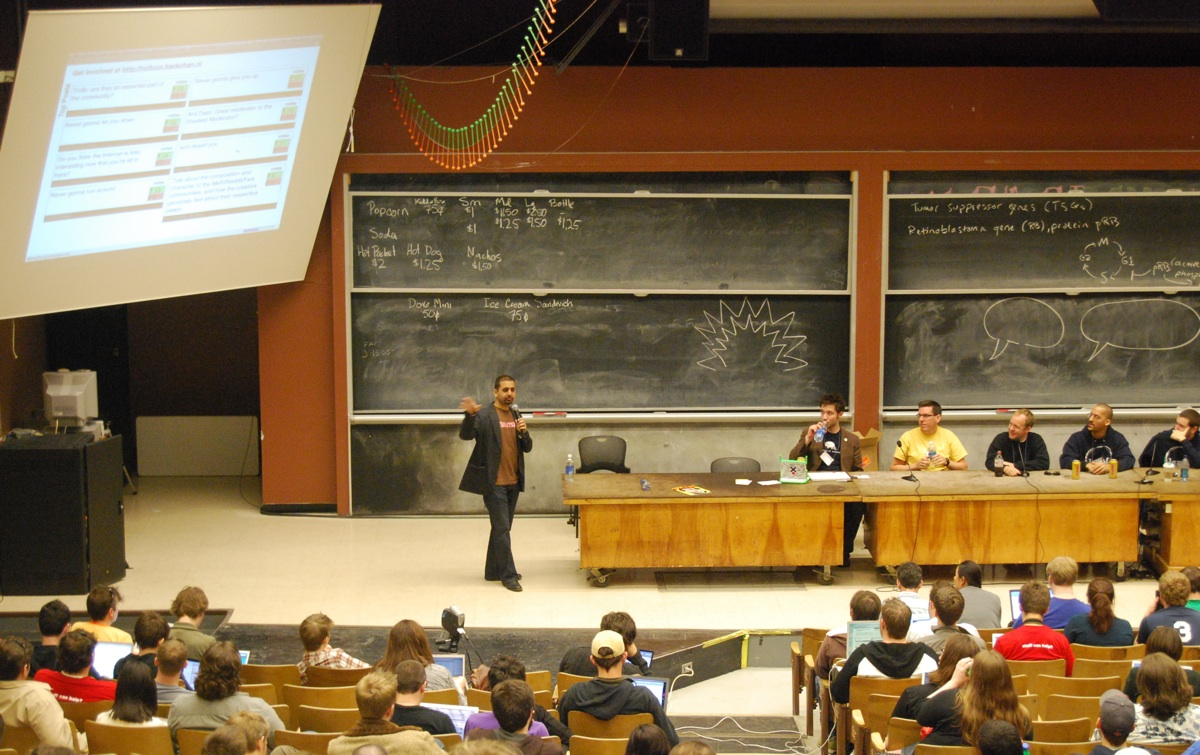
\includegraphics{figures/backchannl/roflcon_photo.jpg}
	\caption{A view of the physical setup for a \emph{backchannl}-enabled event.}
	\label{fig:backchannl_physical}
\end{figure*}

Although the public displays show the top eight posts, the web interface maintains a chronological listing of all the posts that have been submitted during the session. As posts receive positive votes, they tend to rise in the ranking and will eventually reach the top eight and are projected on the main screen. The web interface from which votes are cast and items are submitted can be seen in Figure \ref{fig:backchannl_screenshot}.

When a user first loads the site, they are asked to identify themselves with a name and affiliation. This information is included with any posts that a user made. Votes are publicly anonymous, but are tracked internally with the voter's name to prevent multiple-voting. Identity is easily changed and no formal account registration system is included. The implications of how identity is handled in this system are discussed later in the paper. 

\begin{figure*}[t]
	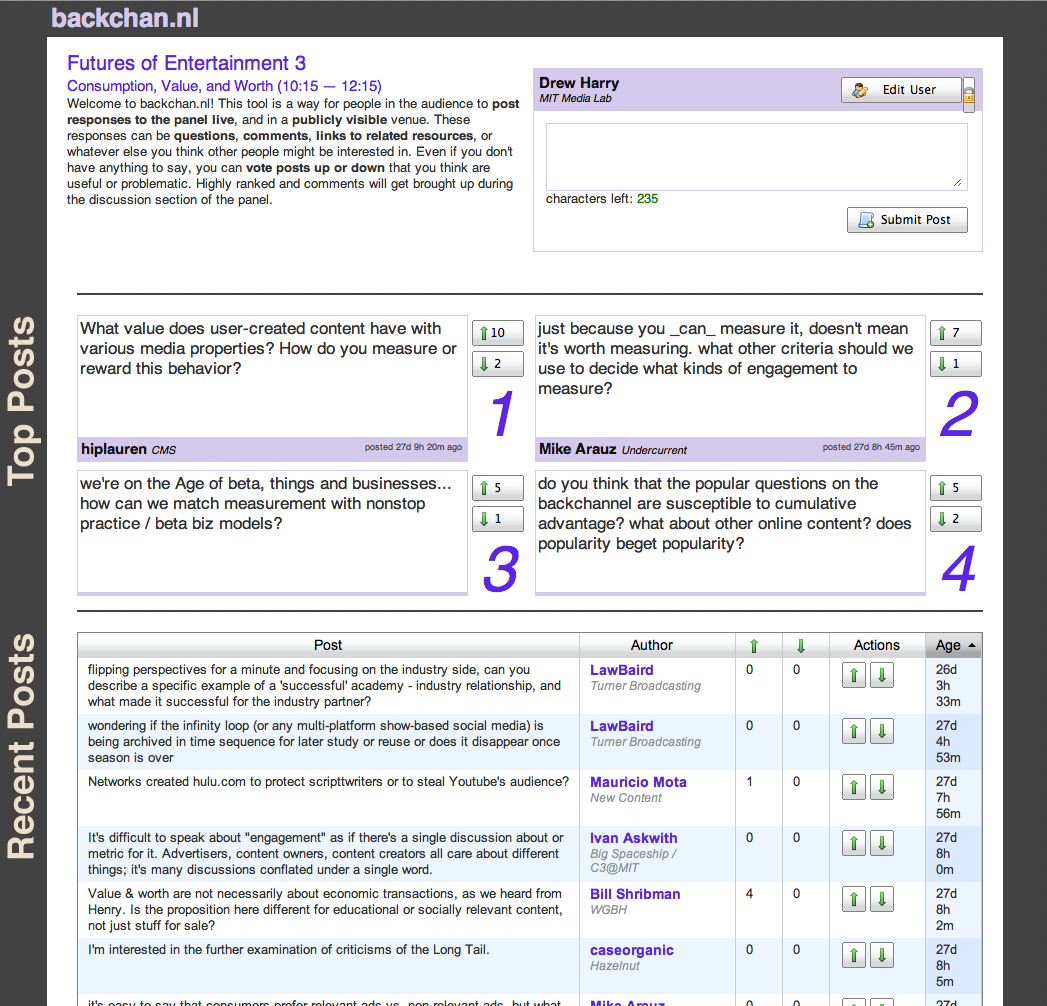
\includegraphics{figures/backchannl/backchannl_screenshot.png}
	\caption{A screenshot of a \emph{backchan.nl} event in action.}
	\label{fig:backchannl_screenshot}
\end{figure*}

\section{Observations}
Although the \emph{backchan.nl} system was designed to be used at one specific event, the success of the tool at that event led to many subsequent inquiries for future deployments. Over the life of the project thus far, \emph{backchan.nl} has been used at hundreds of events. We've had over $14,000$ unique users (though this number is artificially high; see discussions of identity issues in a later section), over $20,000$ items posted, and more than $60,000$ votes cast. The events have included large events with hundreds of audience members and smaller scale events with audiences of fewer than $100$. Most of these events have been panel discussions of some sort, though we have used it for presentation sessions as well.

For our analysis, we will focus on two of our early deployments that share many characteristics but resulted in significantly different experiences. The first event was the Futures of Entertainment 2 conference. This event was our original deployment target, so its structure informed many of our design decisions. The conference was single track and each session was a two and a half hour panel discussion. Panelists gave brief personal introductions, after which discussion amongst panelists was managed by a moderator. The first two thirds of a session were predominantly guided by pre-prepared questions from the moderator, while during the final third, questions were solicited from the audience. We knew from previous years that the conference audience was likely to have large numbers of laptop users and wireless Internet access in the conference venue was known to be excellent. The audience was largely entertainment industry professionals interested in exploring industry issues from an academic perspective.

The second venue was ROFLcon, a two-day conference exploring Internet culture with panel discussions involving significant figures from the Internet community. The convention had multiple tracks, and \emph{backchan.nl} was only used in the biggest presentation space on the second day of the conference. ROFLcon's attendees tended to be much younger than the Futures of Entertainment 2 audience. The ROFLcon audience included many more students and was generally rowdier and more exuberant. It was not uncommon for audience members to interrupt discussion by shouting something at panelists. Anecdotally, this was many attendees' first conference experience. More general descriptions of the atmosphere at ROFLcon can be found in popular media coverage of the event. \citep{Raftery:2008vd}

In terms of their overall format, these two conferences were quite similar; both focused on panel discussions, took place in similarly sized auditorium spaces, and had technically savvy audiences likely to have laptops for accessing the system. Despite this, the audience of each conference used the system in very different ways. In this section, we present and compare usage data between these two conferences.

\subsection{Usage Data--Futures of Entertainment}
Over the course of the five sessions in the conference, there were 125 distinct users. Most names and affiliations were reasonable, with only a handful of obviously anonymous names chosen. The use of pseudonyms or nicknames was generally rare. 

These users posted a total of 224 items, with a mean of 37.6 questions per panel and a mean of 20 questions per each morning introductory session. Across all sessions, we observed a rate of question submission of 0.26 posts per minute and 1.8 posts per registered user over the course of the entire event. We didn't have accurate overall attendance data, but the main hall for the conference has a seating capacity of 190 and was rarely full, so we can conclude that a significant fraction of attendees used the system at some point during the conference.

\begin{marginfigure}
	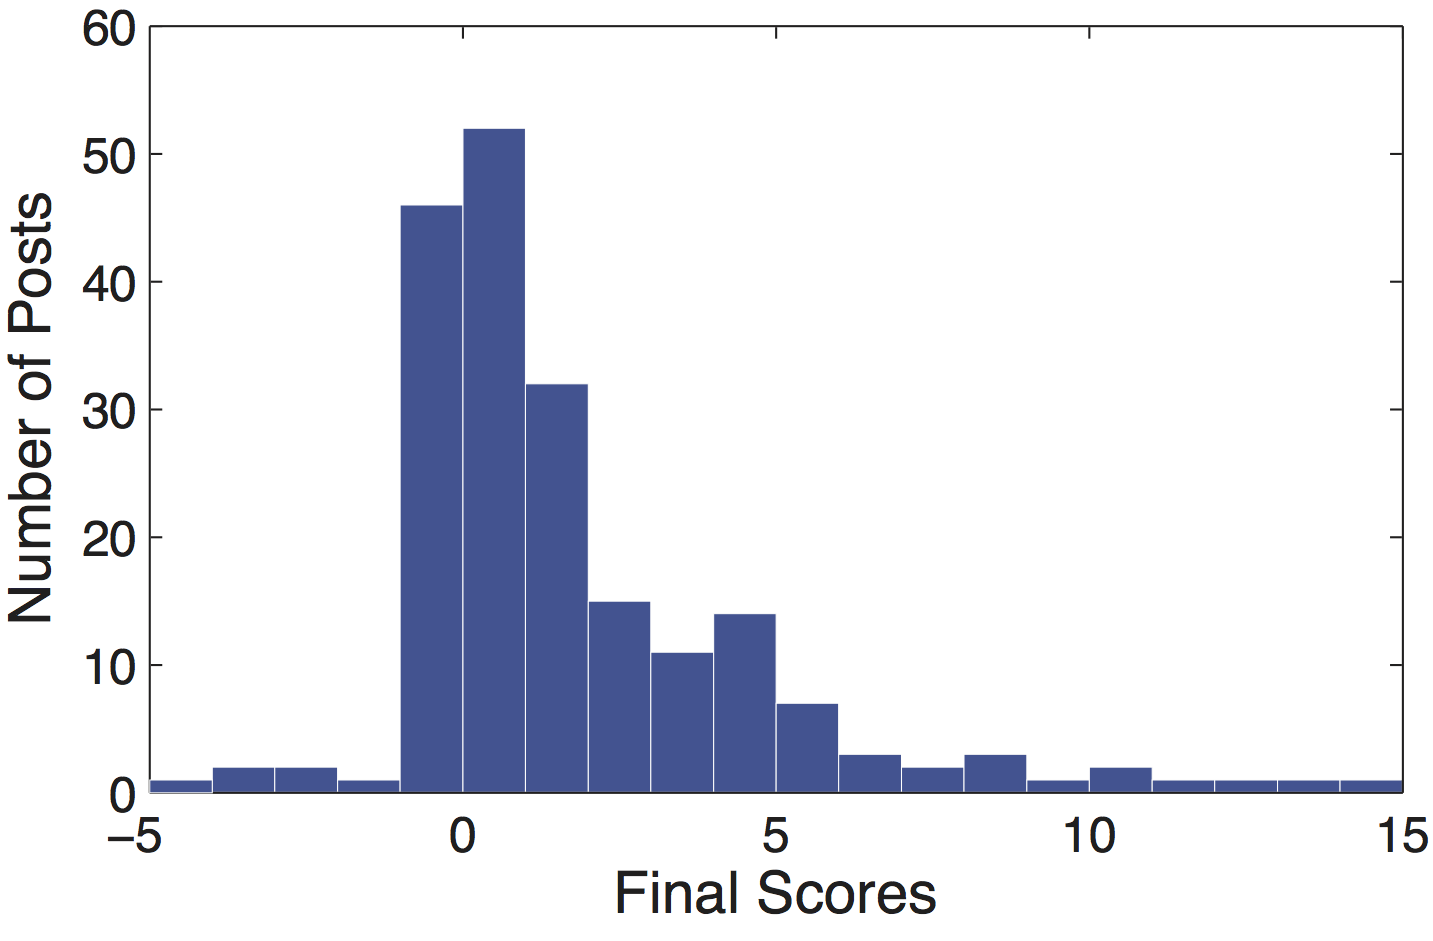
\includegraphics{figures/backchannl/final_scores.png}
	\caption{Histogram of the final scores of posts.}
	\label{fig:final_scores}
\end{marginfigure}

There were a total of 676 votes, with the average post receiving 2 votes. The vast majority of votes were positive: there were 568 positive votes compared to 108 negative votes. The distribution of final scores for posts is shown in Figure \ref{fig:final_scores}. Votes were cast at a rate of 0.78 per minute.



\subsection{Usage Data--ROFLcon}
ROFLcon had five primary sessions that used \emph{backchan.nl}. We observed 450 different usernames, although there are a very large number of pseudonymous names and many duplicate IP addresses recorded. Over the course of those sessions 420 items were posted, at a rate of 1.08 per minute.
There were 1667 distinct votes, recorded at a rate of 4.27 per minute. Of those votes, 1142 were positive, 525 were negative. 



\subsection{Post Contents--Futures of Entertainment}

Over the course of the conference, we observed a number of different categories of posts. Early on in the first panel (and in every subsequent panel), alternative options for audience interaction set up by members of the audience and advertised on the \emph{backchan.nl} system. The first two posts in each panel advertised a Skype public chat and an IRC channel. Private chat was not an inherent feature of our tool, and we were surprised that the first submitted items were advertisements more than questions. In subsequent panels, these postings occurred very quickly, just as the conversation was commencing. Neither channel sustained the same level of involvement as the \emph{backchan.nl} system itself, but its position as a screen visible to all participants in the conference empowered audience-members to create and publicize their own alternative channels. We view the opportunity for the audience to co-opt the channel for competing tools as a demonstration of our commitment to an uncensored channel. Furthermore, such postings highlight the utility of the \emph{backchan.nl} system for audiences to self-organize, and to mediate their own conference experience. These kinds of informational posts didn't score well, and were often the first posts pushed outside of the top eight as soon as questions targeted at the presenters started to be submitted.

During panels, the bulk of popular postings were questions targeted at the panelists. These questions varied in specificity from follow-up questions to panelists (``I would love to hear more about buzz marketing - how it actually works, and how clients want it to integrate it with more traditional methods.") to general synthetic questions (``What's the role of Social Media in advertising and Convergence Culture?").

The other most popular posts represented public sentiment in some way. Near the beginning of the third session, someone posted ``Can we make sure some more questions from the board get answered this time? xthxbai.'' This was the sixth most voted on item in the entire conference. Later in the conference, someone else asked the second most popular question: ``So, is NOW the time the panel should turn some attention to these excellent user-generated questions?'' There was also a complaint about temperature in the auditorium.

Among questions that failed to attract significant attention and votes, there were a number of common themes. Posts that didn't feel sufficiently question-like tended to get passed over. The same was predominantly true for funny and snarky comments. 

\subsection{Post Contents--ROFLcon}
For the most part, items on \emph{backchan.nl} at ROFLcon fall into similar categories as those at Futures of Entertainment. The biggest difference was the balance. There were fewer questions for panelists, but some were certainly generated that were subsequently asked of the panelists, e.g. ``Moot, what is your favorite 4chan meme?'' As at Futures of Entertainment, these items tended to be well received. Most of the top posts in each session were a question for the panelists of some sort.

A significant majority of the posts, however, were not questions. There was a constant flood of jokey posts, for instance: ``WAKE UP SHEEPLE, ALEXIS DID 9/11'', which combines a number of popular Internet memes about a notable community figure (Alexis), a satirical exclamation from the site Alexis runs (``wake up sheeple!'') and 9/11 conspiracies. The success of this kind of post varied widely. Sometimes they were wildly successful, but the vast majority of them languished in obscurity and never made it to the top eight. ROFLcon also had many more announcement type posts like ``::abuses backchannel:: Someone lost a Lumix camera yesterday. Find Susannah on the ROFLTeam to describe it/pics on it.'' As at Futures of Entertainment, messages like these were never highly rated, but did get visibility at the start of sessions. They were rarely submitted later in a particular session. This indicated an understanding that there were phases in a session when different kinds of posts were more or less appropriate. 

ROFLcon's use of \emph{backchan.nl} was much more playful than at Futures of Entertainment 2. This audience was quite familiar with manipulating social tools like this and so pushed the system to its limits. In one session, users engaged in a wide-spread coordinated attempt to rig the item rankings. Eight posts were made containing parts of the lyrics to Rick Astley's ``Never Gonna Give You Up.'' \citep{Anonymous:2007ti} Users then voted these items up and down to make them appear in order in the top eight, attempting to ``rickroll'' the audience. ``Rickrolling'' --- forcing an unsuspecting public to watch/listen to Astley's song --- was a relatively popular Internet meme at the time of the conference. The same user name can't vote more than once on an item, so users participating in this process quickly switched between pseudonyms to trick \emph{backchan.nl} into letting them vote again. When the lyrics were finally in order, someone in the audience yelled ``WE DID IT'' and there was spontaneous applause for their achievement. In this way, users demonstrated a clear internalization of the system dynamics and co-opted the system for their own playful ends. We believe this shows the power of the system that users only play with systems that provide a meaningful stage. Pictures of this happening are available in \citep{Chillag:2008wr}.

\subsection{Voting and Posting Patterns}

\begin{figure*}[t]
	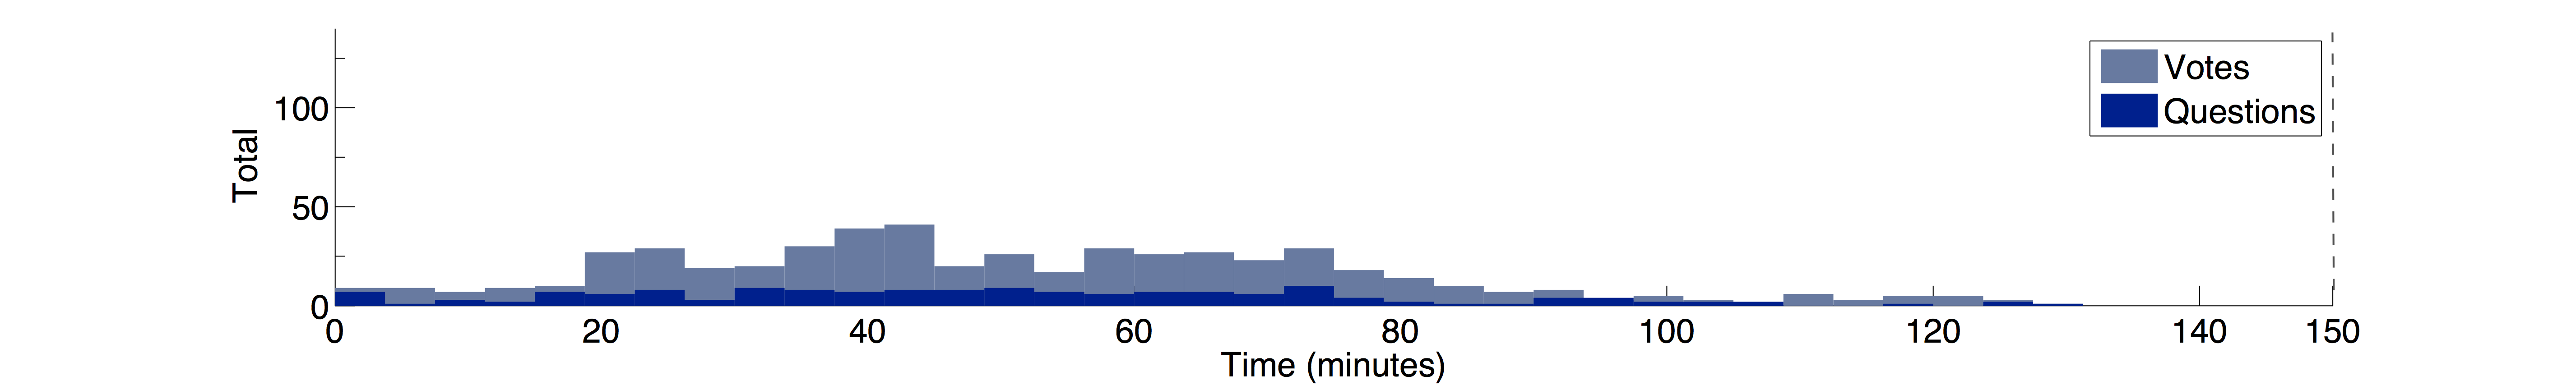
\includegraphics{figures/backchannl/foe2_posting_history.png}
	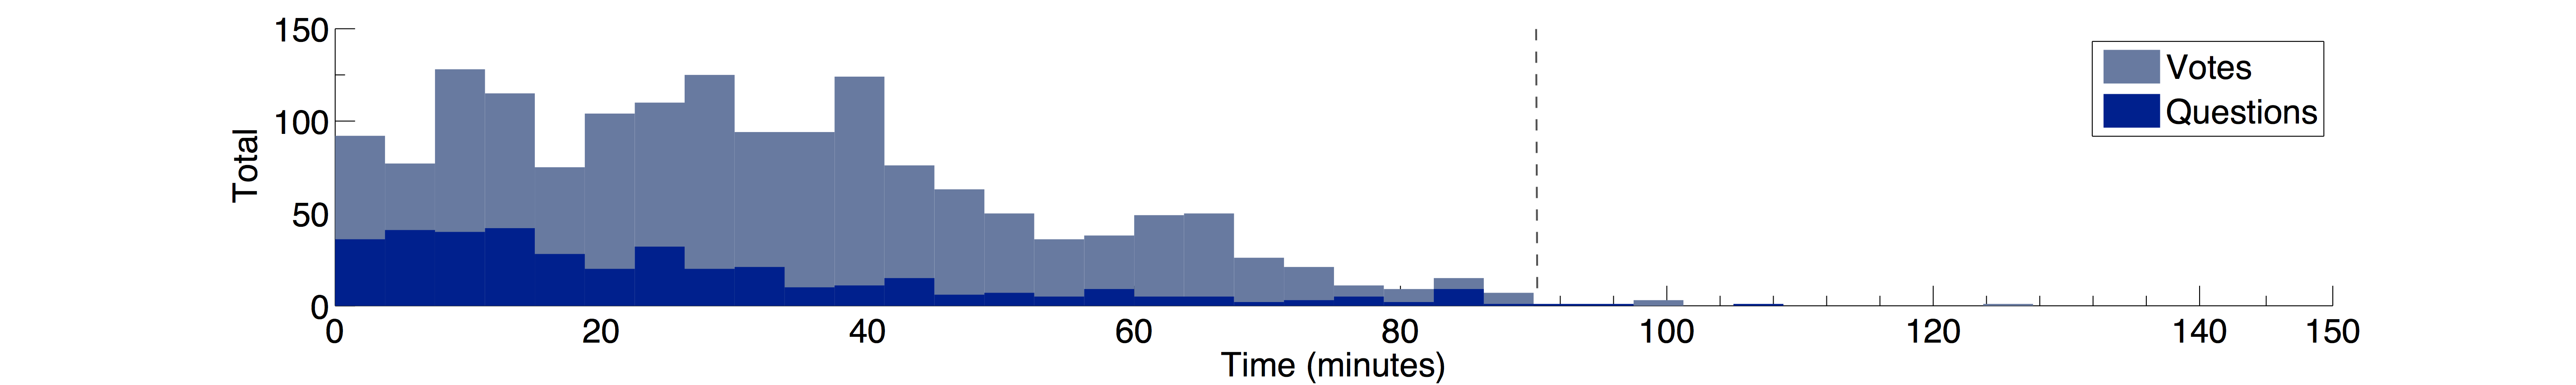
\includegraphics{figures/backchannl/roflcon_figure.png}

	\caption{Accumulated posting and voting events over time. The dashed line marks the duration of sessions in each event. Top: Futures of Entertainment, Bottom: ROFLcon.}
	\label{fig:posting_time_patterns}
\end{figure*}

Over the course of each session, voting and posting patterns emerged that depended quite a bit on the organization of the conference sessions themselves. As seen in Figure \ref{fig:posting_time_patterns}, most of the activity of both posting and voting occurs around the same times. Overall, participation decreases substantially in the second half of every session at Futures of Entertainment 2. This has two possible explanations. Official question time for each panel started between 90 and 120 minutes into each session. Audience members might have chosen to ask questions themselves rather than rely on \emph{backchan.nl} system, given the opportunity. The decline might be a result of users misunderstanding the ranking system and assuming that new posts were unlikely to reach the top eight with so many highly rated posts already submitted. We saw a similar falloff in ROFLcon, though it wasn't as significant. This is closely related to our discussion of tempo later in this paper---it might be the case that this is simply a function of a poor selection of the time constant for these long sessions. 

What is notable about the ROFLcon participation rates is the high number of questions very early on in a session. This is likely because the ROFLcon sessions included public figures the audience was largely already familiar with, and so audience members had questions prepared before the panelists said anything.

\begin{marginfigure}
	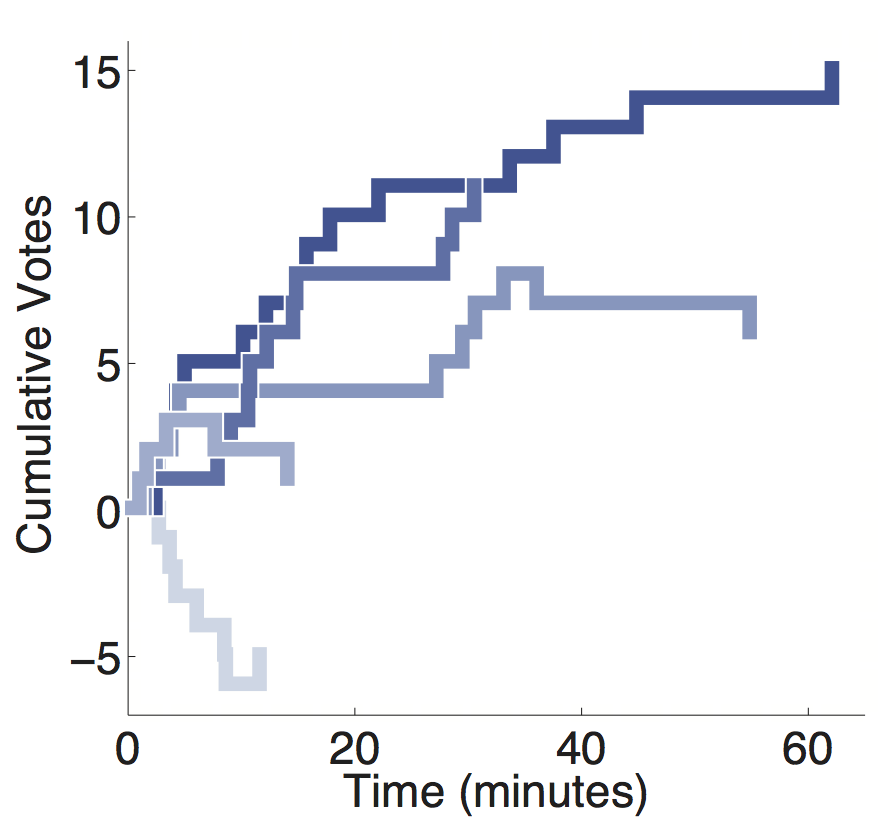
\includegraphics{figures/backchannl/cumulative_vote_histories_colors.png}
	\caption{Tracing the evolution of 5 posts over time. Time 0 is normalized to be the moment the post was submitted. Traces end at the last recorded vote on that item. Notice that the majority of voting on a post happens early in its lifespan.}
	\label{fig:post_score_evolution}
\end{marginfigure}

The voting timelines of a number of different posts are displayed in Figure \ref{fig:post_score_evolution}. In most cases, the voting in the first five minutes of a post's lifetime indicates whether or not it is going to become popular. Posts were rarely contentious---although many posts had some negative votes, they were usually predominantly positive or predominantly negative. These patterns are not unlike those observed in work studying Digg and Reddit, internet-wide systems with a similar voting design. \citep{Lerman:2006wq}


\subsection{Main Stage/Side Stage Integration}
Over the course of the Futures of Entertainment 2 conference, \emph{backchan.nl} was frequently integrated into the foreground conversation. Although the moderators came to each session with a set of prepared questions, most of them quickly went off the script and integrated the posts from the audience into their questions. Often, the moderator would combine a few different questions into a single broader theme and put that question to the panelists. This process was almost always explicit. The moderator would verbally acknowledge the source of the questions, which ones were being combined, and the audience members who asked the original questions. The audience began to expect this kind of behavior and complained when they felt moderators weren't integrating backchannel questions enough. While this also occurred at ROFLcon, the increased non-question ``noise'' meant that moderators had fewer options to choose from. They almost exclusively ignored the funny posts, which really didn't need to be addressed explicitly.

After the Futures of Entertainment event, it became clear that we needed a way to dismiss posts that had been addressed by the moderator. For subsequent events (including ROFLcon) we had some moderation tools that allowed us both to mark a post as answered (reduce its points to zero but still display it in the upcoming list with a checkmark) and ``remove'' a post (remove all user-visible history of the post). The challenges inherent in moderating a system like this are described later in this paper.

Panelists could also see \emph{backchan.nl}, and would sometimes pull questions from it into their responses. This worked particularly well because the panels at both events were very discussion oriented and opened-ended.

This underlines the distinction between traditional ``backchannel'' designs and the main/side stage distinction we aim to create here. With a backchannel approach, integration with the front channel is difficult because the main broadcasters on the front channel have a hard time keeping track of a high frequency backchannel. However with \emph{backchan.nl}, integration was frequent and fluid. This is the goal with side stages, and \emph{backchan.nl} demonstrated it nicely.

\section{User Responses}

In general, users and presenters were very positive about the \emph{backchan.nl} experience. At Futures of Entertainment, conference volunteers conducted interviews with participants after the conference finished, and some participants had comments about \emph{backchan.nl} in particular. One audience member thought ``the ability of people to vote for what they were interested in was great.'' Another participant particularly appreciated that the system ``gave [audience members] opportunities to participate in direct ways.'' Informal chatter at ROFLcon was similar. Moderators tended also to enjoy the system, although they reported having to rethink their moderating approach significantly in light of \emph{backchan.nl}. Over the lifetime of the tool, moderators who have used it more than once are quite positive about its role in panel events, and the organizers of both ROFLcon and Futures of Entertainment requested \emph{backchan.nl} at their next events.

Users and presenters in sessions involving \emph{backchan.nl} expressed a number of common concerns about the system. We collect and address those issues here.


\subsection{Distraction}
The most common concern from presenters was distraction. Some panelists didn't want to use backchan.nl because they thought it would draw attention away from their own comments. We believe that in a space with wireless access, there are plenty of ways for bored audience-members to distract themselves. Indeed, when we watched the screens of audience members, they were rarely staring at the backchan.nl system for long periods of time. They tended instead to bounce between it and many other different websites and applications. This finding is very similar to Golub's observations in \citep{Golub:2005ws}. The projected display itself is intended not to be flashy and attract the attention of people who aren't interested in tracking its content. Still, this is a fair criticism. Although we think this system displays much less information than, say, a modern cable news program, it is still more distracting than non-backchan.nl equipped panels.


In general, users and presenters were very positive about the \emph{backchan.nl} experience. At Futures of Entertainment, conference volunteers conducted interviews with participants after the conference finished, and some participants had comments about \emph{backchan.nl} system in particular. One audience member thought ``the ability of people to vote for what they were interested in was great.'' Another participant particularly appreciated that the system ``gave [audience members] opportunities to participate in direct ways.'' Informal chatter at ROFLcon was similar. Moderators tended also to enjoy the system, although they reported having to rethink their moderating approach significantly in light of \emph{backchan.nl}. Over the lifetime of the tool, moderators who have used it more than once are quite positive about its role in panel events, and the organizers of both ROFLcon and Futures of Entertainment requested \emph{backchan.nl} at their next events. 
Users and presenters in sessions involving \emph{backchan.nl} expressed a number of common concerns about the system. We collect and address those issues here.

\subsection{Presentation Preemption}
Presenters were also concerned that questions would be posted to \emph{backchan.nl} during their presentation that they would answer later in their presentation. Some moderators at Futures of Entertainment 2 expressed concerns that the system placed pressure on them and the panelists to address the audience's concerns first. This concern was also voiced at the handful of non-panel presentations we have run with \emph{backchan.nl}. In these situations, we would typically turn the projection off during the presentation itself and then back on during the question period. During the projection black-out, users could still participate, but the audience as a whole could focus on the presentation materials. Despite presenters' fears, we did not see many instances of the audience pre-empting presentation material with questions.


\subsection{Replies}

Many users lamented the lack of an explicit reply structure in \emph{backchan.nl}. Audience members frequently made explicit comparisons between \emph{backchan.nl} and services like Twitter and IRC, which both have been used in conference situations to provide backchannel conversation. In some deployments these conversations took place over \emph{backchan.nl} itself and became quite contentious. The core complaint in most instances had to do with the lack of a way to distinguish the timing of posts or to indicate that a post was a response to an earlier posting. Some users tried to adopt the ``@username'' format of Twitter, but often these posts would get voted into the top eight without the post it was replying to, decontextualizing the response and confusing audience members who weren't using the tool on a laptop. Over the course of an event, users have almost always moved beyond their initial attempts to use \emph{backchan.nl} in ways it wasn't designed for and settle into a pattern of posting items that aren't explicitly intended to generate responses from the audience. 

In future versions, we would be interested in better affording responses. From a design perspective, we find integrating replies a challenging and interesting problem. Given our limited projection screen space and the contextual nature of discussions, we're hesitant to display elaborate conversations on the screen. Although filtering moderation systems like Slashdot's have been shown to be appreciated by users \citep{Ratto:2003vs}, we have a non-interactive, low density group display and would have to make a global decision for all users about what threshold is appropriate.

We also don't want presenters to feel (accurately or not) that the \emph{backchan.nl} is home to significant conversations that they don't have any visibility into. This is at odds with our desire to have an uncluttered main projection screen. A successful design will have to accommodate both users' desires and presenters' concerns.

\section{Analysis}

What sets \emph{backchan.nl} apart from traditional backchannel approaches is the presence of side stage conversation in the physical space. This approach had a few categories of effects, relative to work on non-physically situated backchannels.

\subsection{Content}
The content in \emph{backchan.nl}'s side stage is markedly different from the content observed in chat-based backchannel implementations \citep{Yardi:2006uk,Cogdill:2001fp,Golub:2005ws,Rekimoto:1998jy}. While the vast majority of posts in this system could be classified as ``Work" messages in McCarthy's categories, they were usually focused on a specific audience --- the panelists. While panelists have sometimes been involved in backchannels in other systems, they knew that the backchannel was largely inaccessible to the main participants on the front channel. Showing \emph{backchan.nl} in the conference space itself makes it clear who is seeing what's posted, and creates the integration that is the signature of a side stage approach. This increases the stakes of communication, as it enjoys an audience that extends to those not actively using the interface itself.

This played out in different ways in the two conferences. For Futures of Entertainment 2, the increased stakes meant users mostly took the system seriously and there were few snarky or critical comments. This is no doubt influenced by the fact many in the audience were attending for professional purposes, either as representatives of their businesses, for networking, or to learn more about their industry. The more playful approach of the ROFLcon audience reflects that community's interests and normal mode of interaction. Higher stakes made users likely to use the system, but content was similar to what they might have normally posted in an online-only discussion. In this way the implementations were not so different; both offered material representations of the different values of the communities present. This echoes the behavior of the children in \citep{Chesnais:uh} who, even in the face of adult disapproval and public attribution of their messages continued to submit messages that the organizers found objectionable. 

\subsection{Adoption}

Adoption is often a serious problem for social systems like \emph{backchan.nl} \citep{Orlikowski:1992tza}. Having a physical representation of audience interaction in the space serves as a constant reminder about how to get involved in the side stage and what is currently happening on it. This provides an effective hook to get new users involved. In particular, the appearance of posts that an audience member thinks is great (or terrible) and the promise that they can help promote or demote it is a powerful incentive. 

The moderators played a key role in \emph{backchan.nl} adoption. After a moderator effectively demonstrates how \emph{backchan.nl} can be used, users quickly build an expectation about its use in future sessions. As with the adoption of other social technologies, it was important for the audience to see that the tool was being taken seriously and that their interactions across it were meaningful to the conference organizers.\citep{Orlikowski:1992tza} This was most clear when the audience co-opted the system to complain about the lack of attention the board was receiving. Indeed, the moderators explicitly responded to each major complaint that appeared on the projection during Futures of Entertainment 2. The chaotic nature of the items at ROFLcon sometimes precluded acknowledgement, though issues with sound were frequently addressed in response to audience comments. 

The physical arrangement in the room further underscores this organizational support. Although people in the audience were able to set up their own backchannels using other software, having a projector and a screen in the room demonstrated the material commitment of the conference organizers to this tool. Although it's possible to imagine situations in which \emph{backchan.nl} might be marginalized by user-organized backchannels, this didn't happen in any of our deployments and we suspect a large part of that is the physical-ness of the design. It's hard to simply ignore a display in the presentation space in favor of a virtual-only conversation space.



\section{Side Stage Configuration}
Based on our experiences deploying the \emph{backchan.nl} system, it has become clear to us that there are a number of ways in which a side stage like \emph{backchan.nl} can be configured that would make this tool both more broadly applicable and more finely tuned for the needs of specific groups of users. In this section, we discuss two major design questions: how should post scores change over time and how should users' identities be represented? In both cases, we argue that a mediated social space like \emph{backchan.nl} would substantially benefit from having configuration options that adapt it to different situations. In much the same way that you might arrange the chairs in a room differently for a lecture versus a group discussion, so too should mediated social spaces have a range of options that foster different social situations.

\subsection{Tempo and Time}

There are a number of modern systems that provide some sort of ``top" list of items. \emph{Digg} and \emph{Reddit} are perhaps two of the most notable (and straightforward) examples of this service; users submit URLs, which can be voted on by other users and by some metric the items are sorted and top items are displayed prominently. These systems (like our system) face an interesting algorithmic challenge: how do you keep the top items changing fluidly such that popular items rise to the top but previously popular items don't linger too long? Certainly, a rank ordering of items by the number of votes is not generally going to be sustainable; older items will tend to accumulate the most votes and make it hard for newly posted items to graduate to the ``top" list of items. In designing a technique for ranking posts, we had a number of goals in mind:

\begin{enumerate}
\item{Highly positively voted posts should get a high ranking.}
\item{New posts should eventually displace older posts.}
\item{Contentious posts should be rewarded somewhat, but less than uniformly well received posts.}
\item{Posts that continue to receive attention over time should stay highly ranked.}
\end{enumerate}

The score is comprised of two factors: an age factor and a vote factor. The vote factor (where $U_p$ and $D_p$ are the up and down votes of a given post p, and where $\overline{(U+D)}$ is the average umber of total votes across all items in the session) is:

\begin{equation}
voteFactor(p) = \frac{kU_p}{U_p + D_p} + \frac{U_p + D_p}{\overline{(U+D)}}
\end{equation}

The first term rewards posts with many positive votes, while the second term promotes items that have a high vote total relative to all posts in the system. In general, the first term rewards positive votes while the second term rewards negative votes. The balance between those terms is set by the constant $k$. 

The age factor (where $t_{p,v}$ is the timestamp of a specific vote on item $p$ and $t_{now}$ is the current timestamp) is:

\begin{equation}
ageFactor(t_p, t_{now}) = \frac{\overline{(t_{now} - t_{p,v})}}{\tau}
\end{equation}

The average time difference was computed for the most recent (up to) five votes on each item. The time constant $\tau$ varied in our experiments, but something on the order of $10^4$ was usually effective.

The two factors are multiplied together to generate the final score.
The main difference between our ranking system and those discussed in \citep{Anonymous:8tu} is that ours measures time not on the basis of the initial posting of an item, but on a moving average of the ages of its votes. In this way, an old item that receives new attention from voters is rewarded.

One of the downsides to this approach is that the points used for internal rankings are not typically made visible to users. This leads to many situations in which an item with few votes is more highly ranked than an older item with many more votes. Although this seems dissonant, users have very rarely commented on it when using the system. Perhaps popular adoption of similar systems has made familiar the notion that voting helps promote something, but that rankings are not strictly tied to votes.

The time constant in the system plays an important role in configuring the space. The time constant sets a sort of tempo for the system; if items decay slowly the top ten is a sort of low-pass filter, showing items that have been of enduring interest to the audience over a long period of a time. This might be useful in a session where the \emph{backchan.nl}'s role is to accumulate questions when there are only a handful of panelists and each panelist speaks for quite a while before there are questions. Conversely, if items decay quickly, the top listing will turn over quickly, exposing a very high-pass view of the audience's interests. This might work well with a panel where the topic is shifting quickly or there are many panelists speaking for a short time. Which kind of time constant is appropriate also has to do with the number of participants. If there are more voters, faster decay makes more sense because more votes will offset the time decay pressure of the ranking equation.

Returning to the goals for a ranking system that we proposed, it is important to note that these goals are specific to the conference situations we were initially designing for. In line with our longer-term interest in describing the ways that a side stage can be configured for different situations, it is easy to imagine conference situations when our goals don't necessarily make sense and we might design a different scoring system. For instance, in a paper-oriented conference like CHI, our goal of having a ``live" list of questions receiving attention might not be appropriate. Instead, a naive ranking mode in which questions accumulate during someone's talk and are ranked purely by their positive and negative votes would be a useful way of identifying the best questions for the end of the talk. This is biased against questions that might be raised towards the end of the talk, but that might actually be valuable. The side stage could act as a counterpoint to the existing structure in which questions often focus on the end of the talk because it's freshest in the audience's mind.


\subsection{Identity}
As in all mediated social systems, how identity is represented in the system can have profound impacts on the behavior in that system. In our design, identity is handled in a very informal way. Users can enter a name and affiliation, but it is trivially easy to change one's personal information. This keeps the threshold for involvement quite low, and we built the system this way to encourage more use. In general, the tradeoff in building identity systems is between low thresholds that encourage use (like our model) and systems that have higher costs to join, but also provide more reliable signals about identity across users. An extreme example of a higher cost identity system might require credentials from a trusted source, but such a system would keep out people who didn't have such credentials or didn't want to expose that much information about themselves. Given our initial venue, we built a system that was biased towards a lightweight identity.

We found (as discussed earlier) that in our first deployment at the Futures of Entertainment 2 conference, there was very little identity play, and our decision promoted productive discussion. This is in stark contrast to ROFLcon, where playful and funny posts outnumbered traditional questions. This playful attitude towards identity is evident in the usage data. There were a much larger number of unique users at ROFLcon of which the vast majority were pseudonymous.

From a design perspective this comparison makes clear that different identity structures make sense for different audiences and presentation structures. When considering the design of future side stage systems, we believe a range of identity options should be offered. Beyond the extremes of no registration and trusted certificates, the system could require email verification or track IP addresses, which would increase the costs to changing identity. In this middle ground, identity in the system is still easily gained, but changing identities is more problematic.

Archiving also plays a role in identity. By changing what kinds of behavior are stored in the system, low-cost identity forms can accrue more costs to changing. If users see other users with rich histories in the system, they will tend to be rewarded for their history by other committed users. \citep{Resnick:2002hf} In this context, users with a history of submitting useful questions can easily be distinguished from someone with a throwaway account. The costs of this kind of pseudonymity have also been explored from a theoretical perspective by\citep{Friedman:2001ti}. Indeed, what about users' behavior is archived and made publicly available is another important axis along which a side stage might be configured.

\subsection{Democracy and Moderation}
This system encodes a basic democratic principle: the best items will rise to the top based on the aggregate will of the audience. There are limits to this principle, though. As mentioned earlier we quickly discovered that we needed some sort of moderation vocabulary. We settled on two basic actions: ``answered'' which sets an item's points to zero and ``remove'' which removes all visible record of the item. Because moderators who used early versions of this system had requested this feature, we hoped that they would also take responsibility for making the decision to demote or remove a post. In practice, this was too much of a burden on them, especially in situations (like ROFLcon) where participants were regularly submitting offensive items, and moderation didn't just involve marking ``answered'' items. 

In practice, one of the authors would sit in the audience and take responsibility for moderating posts. We moderated with a very light hand, marking as answered only those posts that were explicitly mentioned by the moderator and that panelists seemed to answer and removing only those posts that were broadly offensive. Of course, there are substantial grey areas in these criteria. Questions were sometimes posed to panelists and subsequently evaded. Presumably the author of that question would like to see it remain in the top eight, even though the panelist ostensibly responded to it. ROFLcon offered other kinds of posts that we struggled to respond to. In the process of arranging song lyrics in the top eight slots, all other submissions were pushed out. After the ordering was successfully achieved and publicly acknowledged, should we remove them? Indeed, humorous posts in general tended to clog up the top eight because they couldn't really be ``answered'' and so there was no clear contract between the moderator and the audience about how they should be handled. Furthermore, the sheer achievement resonated with the spirit of the conference itself. In the case of the song lyrics, we left them on the board hoping that the audience would subsequently down-vote them to clear the board for new content. This turned out not to be the case, and \emph{backchan.nl} was largely useless for the rest of that panel.

These tensions between keeping the tool effective and letting some version of a democratic process run its course pervade social tools like this. In this case, our approach was to at the very least maintain an open approach to moderation. Posts that were demoted were clearly noted with icons, and all their original votes were still shown on the website view. In this way, the moderator is at least accountable for her actions. In the same way that the audience spoke out against panel moderators who were clearly ignoring \emph{backchan.nl} questions, members could co-opt the tool to protest moderation decisions they disagreed with.

As discussed with respect to tempo and identity, we argue that configuration has an important role to play here. Because the standards and desires of different communities can vary widely, it makes sense in some situations to devolve the moderation controls to the users. Digg, for instance, has systems that allow users to ``bury'' a post they think is inappropriate for some reason. Of course, the risk of tools like this is that they can be easily abused by organized groups of users that want to suppress certain points of view. An effective compromise is ``flagging'' systems used notably by \emph{Craigslist} and \emph{Metafilter}. In this model, users could flag items as being ``offensive'' or ``answered.'' Moderators can use these flags as a proxy for the audience's attitude about specific posts. Having a person making an interpretive decision from this data makes it much harder for groups of users to manipulate an automatic moderation system. There are roles for both of these moderation strategies, as well as the simple benevolent-moderator model we used during our testing. This is the final axis that we propose should be available for configuring side stages. 


\section{Conclusions and Future Work}
In this chapter, we have demonstrated how integrating a side stage into the physical space of a conference can create effective new ways for the audience to interact with panelists, moderators, and other audience members. This approach is in contrast to traditional backchannel systems which focus instead on creating separate audience-only interaction spaces that are somewhat exclusionary to presenters and create a covert character for audience interaction. This shows why chat-based backchannels are viewed as effective for the audience, but rarely integrate well with the front channel. Our posting approach was both a legible interaction metaphor and made \emph{backchan.nl} more appropriate for public projection.

In terms of \emph{in situ} research practice, \emph{backchan.nl} has been a significant success. From its inception, \emph{backchan.nl} was a system whose uses was driven by collaborations with organizations running events with needs specific to those events. After much of this research work was done, the system was extended in such a way that third party organizations could deploy their own \emph{backchan.nl} instances without intervention from anyone on the \emph{backchan.nl} team. The system has seen significant independent use: over 2000 distinct sessions, over 20,000 posts with over 60,000 votes from over 14,000 unique users. This speaks to the extent to which \emph{backchan.nl} accurately addressed a real need in people's lives had a significant impact beyond a lab context. Although not all \emph{in situ} research work should be aimed for broader adoption, we can nonetheless safely argue that broader adoption underlines our claim that we have built something that works in varied social and physical contexts.

There are a number of incremental changes that could be made to improve this system. While the system is currently adapted to posting snippets of text, it could easily be diversified to include many more types of objects. Links to web resources, polls, and discussion threads could all be promoted to first-class objects in the system. An embedded chat interface would also be helpful, providing live discussion opportunities. We are also interested in including some sort of reply mechanism for web-users that does not adversely impact the projected non-participant view. 

More broadly, we're interested in the ways that mediated interaction spaces can be configured for supporting different kinds of social situations. We discuss the ways that tempo and identity function in this particular system as a way of laying out a broader structure for the relationship between these kinds of design decisions and the kinds of interactions they create. 

Finally, we're interested in the potential of side stage systems like this one as a way to involve remote participants with co-located participants. Remote participants are often marginalized and forced to rely on a local advocate to interrupt the flow of conversation and check for questions from remote users. Our side stage approach offers a way to more fluidly involve remote participants by encouraging both local and remote users to interact through the same mediated system. This blurs the lines between local and remote participants and could counteract some of the disadvantages of being a remote participant. Although for the most part the deployments we discuss did not have significant numbers of virtual participants, our future work in this area will explore the implications of this system on remote participants.
